	
	O desenvolvimento deste projeto engloba desde Definição do Escopo do Projeto até o momento de Análise dos Resultados finais, desse modo, para facilitar a organização e controle do Projeto, utilizou-se do apoio do \textit{RoadMap} a seguir:
	
	\begin{figure}[H]
		\centering
		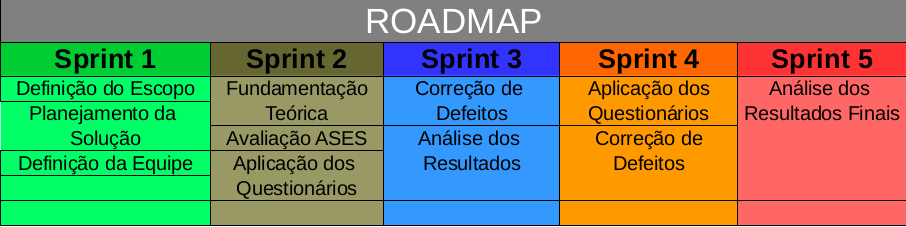
\includegraphics[width=1\textwidth]{imagens/roadmap}
		\caption{RoadMap do Projeto}
		\label{img:roadmap}
	\end{figure}

	Após a conclusão da \textit{Sprint 1}, deve ser possível compreender de forma clara o Objetivo do Projeto, assim como possuir um Planejamento específico sobre como chegar ao Objetivo proposto. Para que durante a \textit{Sprint 2} a Equipe possa obter Fundamentação Teórica em relação à Usabilidade e Acessibilidade de Sistemas Web, e aplicar Questionários de Avaliação nos Usuários do Sistema Enturma.

	A utilização do software \textit{ASES} garantirá a Avaliação da Acessibilidade do Sistema, ainda na \textit{Sprint 2}. Com a obtenção de toda a informação necessária para evolução da Usabilidade do sistema, chega o momento de correção dos defeitos encontrados, que será realizada durante a \textit{Sprint 3}.

	Após a correção, surge a necessidade de avaliar a evolução do sistema Enturma, e com esse objetivo, os Questionários e Entrevistas serão aplicados novamente com os Usuários, durante a \textit{Sprint 4}, para que na \textit{Sprint 5} os resultados possam ser analisados e interpretados.